\documentclass{article}
\usepackage[utf8]{inputenc}

\usepackage{natbib}
\usepackage{graphicx}
\usepackage[]{hyperref}
\usepackage[]{physics}
\usepackage[]{listings}
\usepackage[T1]{fontenc}
\usepackage{color}
\usepackage{float}

\definecolor{mygreen}{rgb}{0,0.6,0}
\definecolor{mygray}{rgb}{0.5,0.5,0.5}
\definecolor{mymauve}{rgb}{0.58,0,0.82}

\lstset{  % requires \usepackage{color} or \usepackage{xcolor}
  backgroundcolor=\color{white},
  basicstyle=\footnotesize,
  breakatwhitespace=false,
  breaklines=true,
  captionpos=b,
  commentstyle=\color{mygreen},
  deletekeywords={...},
  escapeinside={\%*}{*)},
  extendedchars=true,
  frame=single,
  keepspaces=true,
  keywordstyle=\color{blue},
  language=c++,
  otherkeywords={*,...},
  rulecolor=\color{black},
  showspaces=false,
  showstringspaces=false,
  showtabs=false,
  stepnumber=2,
  stringstyle=\color{mymauve},
  tabsize=4,
}

\title{Solving the Schrödinger equation as an Eigenvalue problem}
\author{
  Brandt, Samuel\\
 % \texttt{}
  \and
  Davidov, Aleksandar\\
  \textcolor{blue}{\href{https://github.com/aleksda/FYS4150/}{\texttt{github.com/aleksda}}}
  \and
  Hemaz, Said\\
  % \texttt{}
}
\date{August 2019}

\begin{document}
\maketitle
\begin{abstract}
In this article we are going to solving the Schrödinger equation by rewriting as a matrix problem so that we can use Jacob's method to solve it numerically. What was noticed was that our numerical solution fitted well with the analytical ones. We will discuss three different physical cases in our study. The Buckling Beam problem, and quantum dots in three-dimensions. These cases are different in nature, but the equations to solve them are almost alike, where the only difference is a potential term.
\end{abstract}

\tableofcontents

\newpage

\section{Introduction}
One important problem that occurs in the scientific world is the Eigenvalue problem. They especially play a big role in quantum mechanical systems, which is also the basis for this project, where they are a key part in computations for finding corresponding wave functions. \\
We will in this article first start with a buckling beam problem before we dive into quantum mechanics where quantum dots with both one and two electrons will be studied. 
\subsection{Background}
Even though we are studying different physical problems, the algorithms and even equations needed to solve these problems are identical except for a small potential invariance. \\
Quantum dots is an area of research itself. So far, it has seen use in most notably, LED TVs. One might therefore say that knowing quantum dots and their applications is essensial in the next generation of reaserch.  \\ In order to identify an Eigenvalue problem, one must first have a differential equation of continuous functions in a set interval. We then have to discretize the given equation, then rewrite it as a tridiagonal matrix so we can perform Jacobi's method on it to find the eigenvalues. The reason we take this approach and not the standard pen and paper way, is because that method can become computationally very heavy as the matrix size increases. The way Jacobi's method operates is by iteratively making changes to a matrix until all elements become zero, except the main diagonal. The resulting diagonal will then correspond to the eigenvalues for the original equation. 

\section{Theory}
\subsection{The Equation}

As mentioned, we are going to look at the Buckling beam problem. We start with the differential equation, on the form:
$$l\frac{d^2u(x)}{dx^2} = -Fu(x)$$
Where $u(x)$ is defined as the vertical displacement for the beam in the $y$ direction. The beam has length $L$, and $F$ is the force applied at the points $(L,0)$, in direction towards the origin. Further, $l$ is the constant defined by properties like the rigidity of the beam. In this project, we have set the Dirichlet boundary conditions $u(0)=u(L)=0$. In our case, the parameters $l$, $F$ and $L$ are known. We therefore define a dimensional variable $$\rho=\frac{x}{L}$$ so we have $\rho \in [0,1]$. This will give us the equation $$\frac{d^2u(\rho)}{dp^2}=-\frac{FL^2}{R}u(\rho)=-\lambda u(\rho)$$ This means $\lambda =\frac{FL^2}{R}$. Further, the approximation to the second derivative will give us
\begin{equation}
u''=\frac{u(\rho +h)-2u(\rho)+u(\rho -h)}{h^2}=O(h^2)
\end{equation}
where $h$ is the step length. Next we define maximum and minimum values for $\rho, \rho_{max}, \rho_{min} =0$. With a given number of mesh points,$N$, we define the step length $h$ as $$h=\frac{\rho_n-\rho_0}{N},$$ where $\rho_{max}=\rho_N$ and $\rho_{min}=\rho_0$. The values of $\rho$ at point $i$ is then $$\rho_i=\rho_0+ih \hspace{1cm}i=1,2,\dots,N.$$ The entire equation can be rewritten as $$
-\frac{u(\rho_i+h) -2u(\rho_i) +u(\rho_i-h)}{h^2}  = \lambda u(\rho_i),$$ or in a little more compact way as $$-\frac{u_{i+1} -2u_i +u_{i-1} }{h^2}  = \lambda u_i.$$ This equation can be rewritten in a much more compact form, a form that will make it easier for us to solve it, that is
\begin{equation}
    \begin{bmatrix} d& a & 0   & 0    & \dots  &0     & 0 \\
                                a & d & a & 0    & \dots  &0     &0 \\
                                0   & a & d & a  &0       &\dots & 0\\
                                \dots  & \dots & \dots & \dots  &\dots      &\dots & \dots\\
                                0   & \dots & \dots & \dots  &a  &d & a\\
                                0   & \dots & \dots & \dots  &\dots       &a & d\end{bmatrix} 
                                 \begin{bmatrix} u_1 \\ u_2 \\ u_3 \\ \dots \\ u_{N-2} \\ u_{N-1}\end{bmatrix} = \lambda \begin{bmatrix} u_1 \\ u_2 \\ u_3 \\ \dots \\ u_{N-2} \\ u_{N-1}\end{bmatrix} . 
\label{eq:matrixse} 
\end{equation}
Here, we do not include the endpoints $u_0$ and $u_N$. We have defined the diagonal $d=2/h^2$ and the non-diagonal $a=-1/h^2$.
We know that this eigenvalue problem has analytical eigenpairs, with eigenvalues given as 
\begin{equation}
\lambda_j=d+2a\cos{\frac{j\pi}{N+1}}\hspace{1cm}j=1,2,\dots,N
\end{equation}

This approach for discretizing a given equation and setting it up as a tridiagonal matrix is very similar for quantum dots in two and three dimentions. But for times sake, the approach will not be shown in this article. Interested readers may refere to reference number 1 in the bibliography.

\subsection{Short note on orthogonality}
Now, before we continue, I am going to tell a little about orthogonality. So, in basics terms, two vectors $u$ and $v$ are orthogonal if they are linearly independent. In other words if they are perpendicular to each other. Now consider the vector

\[
\mathbf{v}_i = \begin{bmatrix} v_{i1} \\ \dots \\ \dots \\v_{in} \end{bmatrix}
\]
We are going to prove that a unitary transformation preserves the dot product and orthogonality. 
We assume that the basis is orthogonal, that is 
\[
\mathbf{v}_j^T\mathbf{v}_i = \delta_{ij}.
\]
We have the transformation
\[
\mathbf{w}_i=\mathbf{U}\mathbf{v}_i,
\]
where $\mathbf{U}$ is a unitary matrix such that $\mathbf{U}^T\mathbf{U}=\mathbf{I}$. Since $\mathbf{w}$ is the unitary transformation, we have to prove that $\mathbf{v}_j^T = \mathbf{w}_i^T$. 
$$\mathbf{w}_i^T \mathbf{w}_j=(\mathbf{Uv}_i)^T\mathbf{Uv}_j=\mathbf{v}_i^T\mathbf{U}^T\mathbf{Uv}_j,$$ since $\mathbf{U}^T\mathbf{U}=\mathbf{I}$ we get 
$$\mathbf{v}_i^T\mathbf{I}\mathbf{v}_j=\mathbf{v}_i^T\mathbf{v}_j=\delta_{ij},$$ thus we have proven that a unitary transformation preserves the dot product and orthogonality. \\
This theorem is important for the next part in our project!

\section{Algorithm}
\subsection{Jacobi rotation algorithm} In this part we are going to implement the Jacobi rotation algorithm to solve Eq. (2). But first, we are going to set up the matrix and diagonalize it with a given number of mesh points, N. Then compare the numerical eigenvalues to the analytical ones. To do this, we first set up the matrix using the Armadillo library for C++. We start by defining the variables like N, $\rho_N$, $\rho_0$ and $h$. As we saw in the theoretical part, we define $h=\frac{\rho_N-\rho_0}{N}$ and the diagonal $2/h^2$ and non-diagonals as $-1/h^2$. Then we start to make an empty NxN matrix, give it first element equal to $d=2/h^2$ and second element equal to $a=-1/h^2$. The last part of the matrix is to use a for-loop to fill out the remaining elements up till $N-1$. \\
Now, we make a vector with dimensions N, and use the command $\textit{eigsym}$ from Armadillo to find the eigenvalues. Lastly, we define function for the analytical eigenvalues from Eq. (3). and print out the absolute value off the numerical ones - the exact ones. \\
What we see is that the numerical eigenvalues is correct to 14 decimal-places. That's impressive! \\ \\
Now, our next part is to implement the Jacobi rotation algorithm. To do this, first consider these two (2x2) matrices
\begin{equation}
A = \begin{bmatrix}
a_{11} & a_{12} \\
a_{21} & a_{22}
\end{bmatrix}
\end{equation}
and,
\begin{equation}
R = \begin{bmatrix}
c & -s \\
s & c
\end{bmatrix}
\end{equation}
Where the matrix A is symmetric and the matrix R is a rotation matrix. This means that when multiplied with a vector $\mathbf{v}$, rotates around an angle $\theta$. In the matrix (5), we have made the substitution $c=\cos{\theta}$ and $s=\sin{\theta}$. The matrix $R$ (or any rotation matrix for that matter) has properties $R^T=R^{-1}$ We can now wire a similarity transformation $R^{-1}AR$. This transformation is also symmetric, but I will not show that. This matrix needs to be rotated in a way so all non-diagonal elements become zero. That means we would need to take the non-diagonals equal to zero. The non-diagonal are $$\frac{a_{11}-a_{2}}{2a_{12}}=\cot{2\theta}=\tau.$$ Now if we set $t=\tan{\theta}$, and use $cot{2\theta}$. we obtain the quadratic equation $$t^2 + 2\tau t -1 = 0,$$ putting t on the left side, we get $$t=\tau \pm \sqrt{1+\tau^2}.$$ The c and s can now obtained,$$c=\frac{1}{\sqrt{1+t^2}}$$ and $s=ct$. Now after solving $\tau$ our similarity transformation matrix will then look like this
$$
R^{-1}AR = \begin{bmatrix}
a_{11} & 0 \\
0 & a_{22}
\end{bmatrix}
$$

Code snippet in C++ for the main part of the algorithm is shown bellow.
\begin{lstlisting}
if(A(k, l) != 0.0){
        double tau;
        tau = (A(l, l) - A(k, k)) / (2 * A(k, l));

        double t;
        if (tau >= 0) {

            t = 1.0 / (tau + sqrt(1 + pow(tau, 2)));

        } else {

            t = -1.0 / (-tau + sqrt(1 + pow(tau, 2)));
        }
        // Sine and cosine
        c = 1.0 / (sqrt(1 + pow(t,2)));
        s = c * t;

    // Division by zero
    } else {
        s = 1.0; c = 0.0;
    }

...

for (int i = 0; i < dim; i++) {
        if (i != k && i != l) {
            //a_ik, il etc is value of A(i, k), etc
            a_ik = A(i, k);
            a_il = A(i, l);
            A(i, k) = a_ik * c - a_il * s;
            A(k, i) = A(i, k);
            A(i, l) = a_il * c + a_ik * s;
            A(l, i) = A(i, l);
        }
\end{lstlisting}


\section{Results}
First we started making the tridiagonal matrix and then diagonalized it. What we noticed was that the numerical computation was very precise. The fact that we already had the analytical solutions in this project, made testing a lot more simple and it gave something to look after. However, for the quantum mechanics part, it was intuitive to know what the radial solutions whould look like for the different eigenstates in the harmonic oscillator potential. Figure \ref{fig:dotone} show the eigenstates with the lowest values for the harmonic oscillator with one electron.
\begin{figure}[H]
\centering
%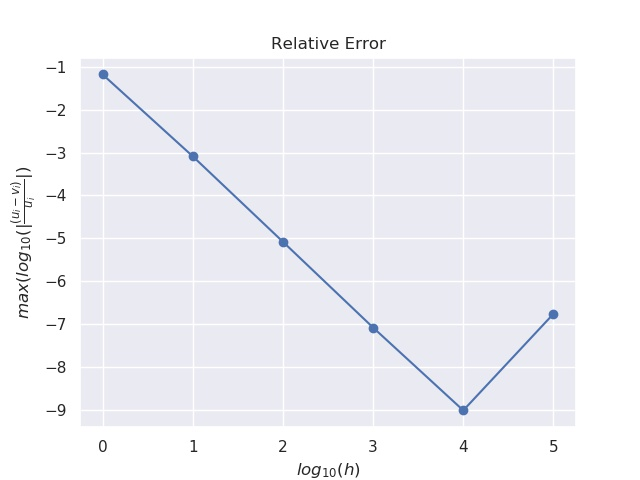
\includegraphics[scale=1.7]{error.png}
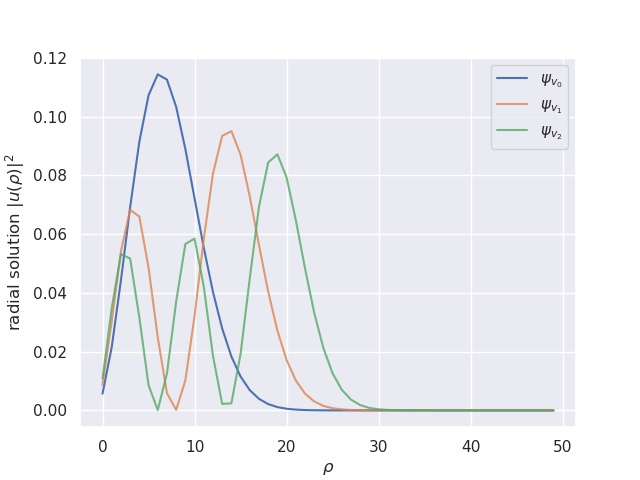
\includegraphics{quantumdot_one.jpg}
\caption{Three lowest eigenstates in one dimension}
\label{fig:dotone}
\end{figure}

Comment about the unsmoothness: I am using an old laptop at the time I computed the eigenvector. in Figure \ref{fig:dotone} the value $\rho_{max}$ was simply just $1.0$. The way this plot was made was using the "Armadillo" linear algebra library for C++. Armadillo's function 'arma::eigsym()' can return the eigenvectors of a given matrix. This approach wass chosen because purpose for this project was to find the eigenvalues numerically, therefore using Armadillo was used for eigenvectors to speed up the development 

\section{Conclusion}
\citep{Project2}

\bibliographystyle{plain}
\bibliography{references}
\end{document}

